\chapter{Tune procedure, CP5 Tune and \textsc{mcnntunes}}
\label{chap:TuneprocedureCP5TuneandMCNNTUNES}

The study of the underlying event, or more in general of softQCD processes require the use of Monte Carlo generator based on phenomenological model all these models introduce lot of free parameters that must be tuned on experimental data in order to obtain meaningful results. The procedure of estimate the best parameters values is called \textit{tune}. 

The tune procedure can be really computational expensive,  can require to run the generator a very large amount of times. And usually these MC generator are really expansive in computation time required for a single job. 

To tune some parameters the number of jobs you have to run increase with the number of parameter you want to tune. different approaches have been used in the past to tune these MC generator:
\begin{enumerate}[label=\arabic*)]
	\item \textbf{Manual tunes}: this approach is based on an optimization of the parameters made by eye. This is absolutely not the best way to tune some parameters, usually it requires a very large time for even semi-reasonable results since the process require a very large number of iterations.   
	\item \textbf{Brute force tunes}: A better way would be to perform a very dense sampling in parameters space and run a generator with every configuration. This is very computational expensive and a scan in a 5 parameters space with 10 division each require 100000 Monte Carlo runs this is really impractical.   
	\item \textbf{Parametrization-based tunes}: An even more better approach is to find a surrogate function to parameterize the response of the MC generator at different values of the parameters to tune and try to study (minimize) this surrogate function instead of the real response of the generator.
\end{enumerate}

\section{Parametrization-based approach}

The last one is the most used the current state-of-art in the tune procedure is to use a polynomial function to fit the response of the generator and minimize it, this approach is implemented in the software \textsc{Professor} \cite{Buckley:2009bj}. 

The first step in the procedure is to fit the response of the generator using a surrogate function simpler to study,
\begin{equation}
	h(p)\ \xrightarrow{\quad \text{parametrization}\quad }\ \overline{h}(p)
\end{equation}
than a \textit{loss function} $\mathcal{L}(h(p),h_{\text{data}})$ is defined, between the surrogate function and the experimental data, a common choice is the $\chi^2$ function defined as:
\begin{equation}
	\mathcal{L}(h(p),h_{\text{data}})\equiv \chi^2=\frac{(h(p)-h_{\text{data}})^2}{\sigma}
\end{equation}
Than to find the best parameters estimation this loss function need to be minimized, the set of parameters $p_{\text{best}}$ that do this are the best evaluation that our generator can provide for the real values and are our \textit{tune}.
\begin{equation}
	p_{\text{best}}=\arg\,\min_p\ \mathcal{L}(h(p),h_{\text{data}})
\end{equation}

In our study instead of the common software \textsc{professor} based on the polynomial parameterization we use the machine learning approach implemented in \textsc{mcnntunes} software %%%CITARE%%%
with Feed Forward Neural Networks. \textsc{mcnntunes} is a software developed by S. Carazza, S.Aioli and M.Lazzarin \cite{MCNNTUNESarticle} based on machine learning library TensorFlow \cite{tensorflow2015-whitepaper}. \textsc{mcnntunes} is write in pyhton and it uses neural networks (NN) that are trained to learn the generator behavior to the parameter values.

Let's make a brief introduction on machine learning and in particular on neural networks

\section{Machine Learning and Neural Networks}
  
Machine learning (ML) is a particular type of Artificial Intelligence it consist in systems that learn automatically by the data that are feed to it and not by the explicit programming of the algorithm. Is clear that the machine learning require the training of the algorithm in order to have a prediction on the problem under analysis.

A particular type of ML is Deep Learning that uses neural networks with more than one layer organized in a hierarchical structure.

\subsection{Neural Networks - Perceptron}

The concept of the neural network was developed in 1958 by Frank Rosenblatt. He introduce the simpler example of NN: the perceptron \cite{Perceptron}. A representation of a percepton is shown in \figRef{fig:Perceptron} the input values are weighted and summed than the weighted-sum is passed to an activation function (step function) an additional offset $b$ can be introduced, the output of the perceptron is than:
\begin{equation}
	h(x)= \text{step}(w^T\, x + b)
\end{equation}

\begin{figure}[!ht]
	\centering
	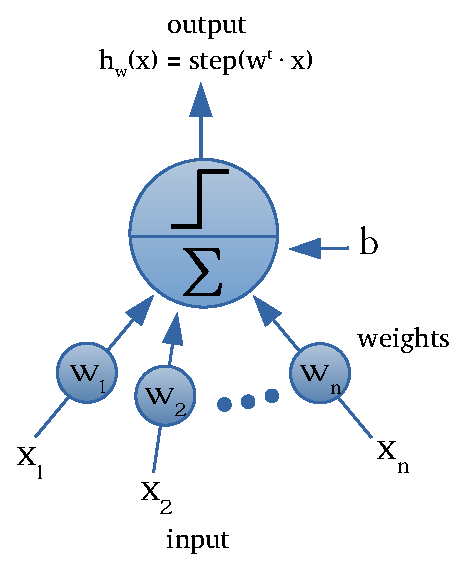
\includegraphics[scale=0.7]{{img/Perceptron2.pdf}}
	\caption{A schematic representation of a perceptron.}
	\label{fig:Perceptron}
\end{figure}

The revolutionary feature of the perceptron was the ability of learning by an adjustment of the weights. But a single perceptron is not enough. An example of limitation in shown in \figRef{fig:XORproblem} where the impossibility of implement a \textsc{xor} operation using a perceptron is shown with a graphical explanation. The perceptron is a linear classification algorithm and in the image is draw as a line that set a boundary for the acceptation of the hypothesis.

\begin{figure}[!ht]
	\centering
	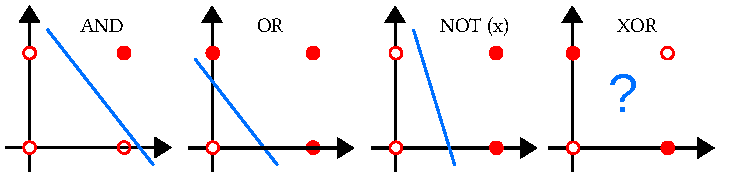
\includegraphics[width=14cm]{{img/XORproblem.pdf}}
	\caption{The figure shows one of the limitations of the perceptron the }
	\label{fig:XORproblem}
\end{figure}

The structure is very simple with a single unit but is not enough it have a lot of limitation so we have to introduce the concept of NN with more than one unit.

\subsection{Feed-Forward Neural Networks}

different units call "neurons" are linked together to compose an artificial NN. There are  different type of NN we are interested in Feed-Forward NNs and fully-connected that are the ones used in \textsc{mcnntunes}. 

\figRef{fig:NNesample} show a schematic view of a NN the basic idea is that the neurons can get some value in input and return a value as output, in fully-connected NN each neurons from a layer are connected to every neurons in the next layer. As we will discuss later one of the biggest feature of the NNs is that the they are universal function approximators \cite{HORNIK1991251, LESHNO1993861} the only request is that a sufficient number of hidden layer is available.

The Feed Forward attribute refers to the fact that the NN don't have internal recursion (loops) between neurons.

\begin{figure}[!ht]
	\centering
	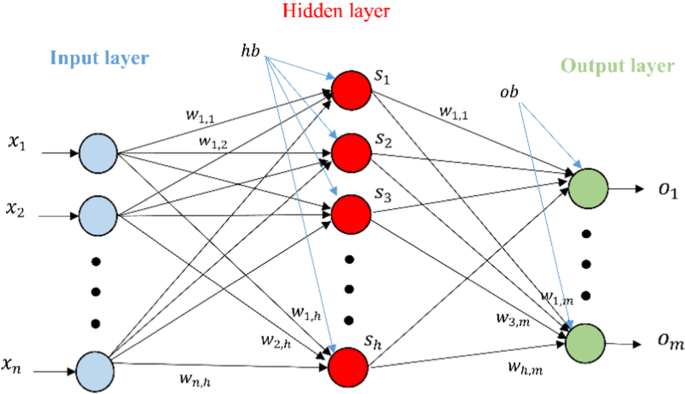
\includegraphics[width=14cm]{{img/NNesample.png}}
	\caption{A fully-connected feed-forward neural network}
	\label{fig:NNesample}
\end{figure}

A common training algorithm for the NN is the back-propagation. A set of Monte Carlo simulation is used to train the NN. The procedure is based on the idea of change the weights $w_{jk}$ and parameters $\vartheta_{j}$ in order to minimize a loss function usually defined as the mean squared error ($E$):
\begin{equation}
	E=\frac{1}{2}\displaystyle\sum(h_{i}(x^j,w_{jk})-d_i)^2
\end{equation}  
where the $h_{i}$ are the value in output from the NN and the $d_{i}$ the real value known from the Monte Carlo truth.

In the back-propagation algorithm the weight and the coefficients are update using the steepest-descent minimization:
\begin{equation}
	w_{jk}^{(i+1)}=w_{jk}^{(i)}-\lambda\left( \frac{\partial E}{\partial w_{jk}} \right)^{(i)}
	\qquad\qquad
	\vartheta_{j}^{(i+1)}=\vartheta_{j}^{(i)}-\lambda\left( \frac{\partial E}{\partial \vartheta_{j}} \right)^{(i)}
\end{equation}
where $\lambda$ is the learning rate and is a user-tunable free parameter. 

The batch is our training set that contains the Monte Carlo simulation that is used to calculate the gradient. The size of the batch used to train the NN is also a free parameters: smaller batch are faster to compute but the direction is not the real one but an approximation while, bigger batch size give a good approximation of the direction of the steepest-descent but can be computational expensive. 

The number of evaluation of the entire batch is called epochs and is tunable by the user.

The batch size and the number of epochs are related. A batch of 50 run with a batch size of 10 and a number of epochs of 1000 require 5000 iterations while if we use a batch size of 25 it require only 2000 iterations to run over all the training set.

\begin{figure}[!ht]
	\centering
	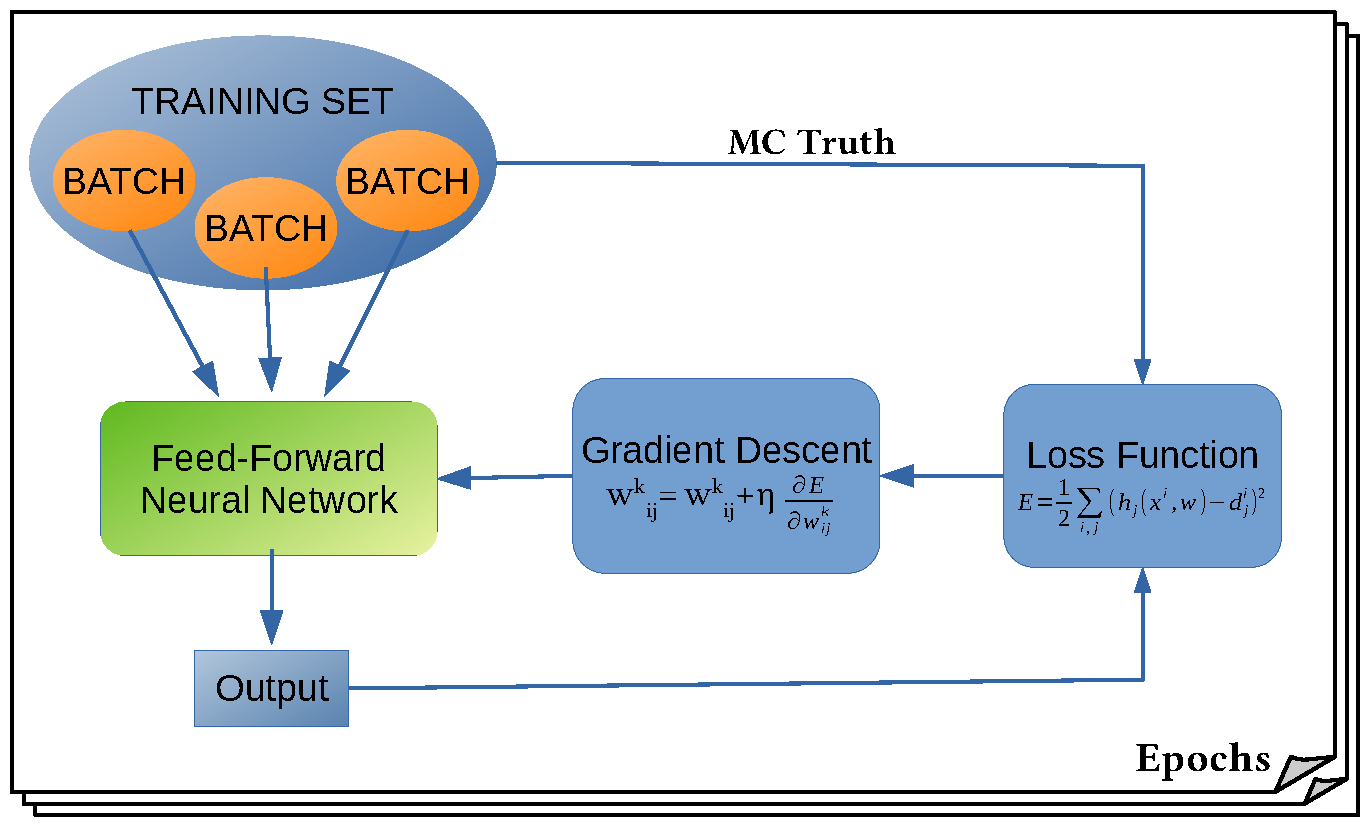
\includegraphics[width=14cm]{{img/Training2.pdf}}
\end{figure}

\section{Previous Tune for the Underlying Event}

In the paper \cite{CPtunes} the CMS collaboration presents new \textsc{pythia8} tunes for the underlying event. The tunes are called CP and a number from 1 to 5 where CP stands for \textsc{"cms pythia8"}. The tunes are performed changing the values of the coupling constant $\alpha_s$ for the ISR, FSR, hard scattering and MPI and the order of the evolution with the value of $Q^2$ for the interaction. Another difference among these tunes is the choice of the PDF set. The parameter that are tuned are shown in \tableRef{table:CP5variations} with the associated variation ranges. 

\begin{table}
	\centering
	\resizebox{0.97\textwidth}{!}{
	\begin{tabular}{l c c}
		Parameter description & Name in PYTHIA8 & Range considered\\\hline\hline
		\\[-8pt]
		MPI threshold $[\mathrm{GeV}]$, \texttt{pT0Ref}, at $\sqrt{s}=\sqrt{s_0}$ \ & \texttt{MultipartonInteractions:pT0Ref} &  $1.0-3.0$ \\[3pt]
		Exponent of $\sqrt{s}$ dependence, $\epsilon$ & \texttt{MultipartonInteractions:ecmPow} & $0.0-0.3$ \\[3pt]
		Matter fraction contained in the core & \texttt{MultipartonInteractions:coreFraction} & $0.1-0.95$ \\[3pt]
		Radius of the core & \texttt{MultipartonInteractions:coreRadius} & $0.1-0.8$ \\[3pt]
		Range of color reconnection probability & \texttt{ColorReconnection:range} & $1.0-9.0$ \\[3pt]
	\end{tabular}
	}
	\caption{This table report the five parameters tuned for the underlying event in CP tunes, the variation ranges used for the sampling are shown in the last column. Table from \cite{CPtunes}}
	\label{table:CP5variations}
\end{table}

\subsection{The distributions used}
\label{sec:Thedistributionsused}

The observables distributions used for the tune are the following one:

%\begin{table}
%	\centering
%	%\resizebox{\textwidth}{!}{
%	\begin{tabular}{l l}
%	Rivet Analysis & Distribution\\\hline\hline
%	\\[-8pt]
%	CMS\_2015\_I1384119 & d01-x01-y01\\[2pt]
%	CMS\_2015\_PAS\_FSQ\_15\_007 & d01-x01-y01\\[2pt]
%	CMS\_2015\_PAS\_FSQ\_15\_007 & d02-x01-y01\\[2pt]
%	CMS\_2015\_PAS\_FSQ\_15\_007 & d05-x01-y01\\[2pt]
%	CMS\_2015\_PAS\_FSQ\_15\_007 & d06-x01-y01\\[2pt]
%	CMS\_2012\_PAS\_FSQ\_12\_020 & d05-x01-y01\\[2pt]
%	CMS\_2012\_PAS\_FSQ\_12\_020 & d06-x01-y01\\[2pt]
%	CMS\_2012\_PAS\_FSQ\_12\_020 & d08-x01-y01\\[2pt]
%	CMS\_2012\_PAS\_FSQ\_12\_020 & d09-x01-y01\\[2pt]
%	CDF\_2015\_I1388868 & d01-x01-y01\\[2pt]
%	CDF\_2015\_I1388868 & d02-x01-y01\\[2pt]
%	CDF\_2015\_I1388868 & d05-x01-y01\\[2pt]
%	CDF\_2015\_I1388868 & d06-x01-y01\\[2pt]
%	CMS\_2018\_I1680318 & d01-x02-y01\\[2pt]
%	CMS\_2018\_I1680318 & d01-x03-y01\\
%	\end{tabular}
%	%}	
%\end{table}

\begin{itemize}
	\item The pseudorapidity distribution of charged hadrons ($p$, $K$ ,$\pi$) measured for an
inclusive selection in inelastic proton-proton collisions
\item Charged particle density and charged particle scalar $p_T^{sum}$ in TransMIN and TransMAX regions at different $\sqrt{s}$ ($1.96\ \mathrm{TeV}$, \, $7\ \mathrm{TeV}$, \, $13\ \mathrm{TeV}$)
\item The pseudorapidity distributions for single diffractive (\textsc{sd}) and non single diffractive (\textsc{nsd}) events selection
\end{itemize}
In the next chapter we will describe our tune using \texttt{mcnntunes} and in it we used the same distribution listed here.

\subsection{Pyhtia configuration and the tunes}

On the top section of \tableRef{fig:CPtunes1} and \tableRef{fig:CPtunes2} are reported the values for the \texttt{pythia8} parameters used in the CP tunes and, on the bottom, the 5 parameters resulting from the tune.

\begin{table}[!ht]
	\centering
	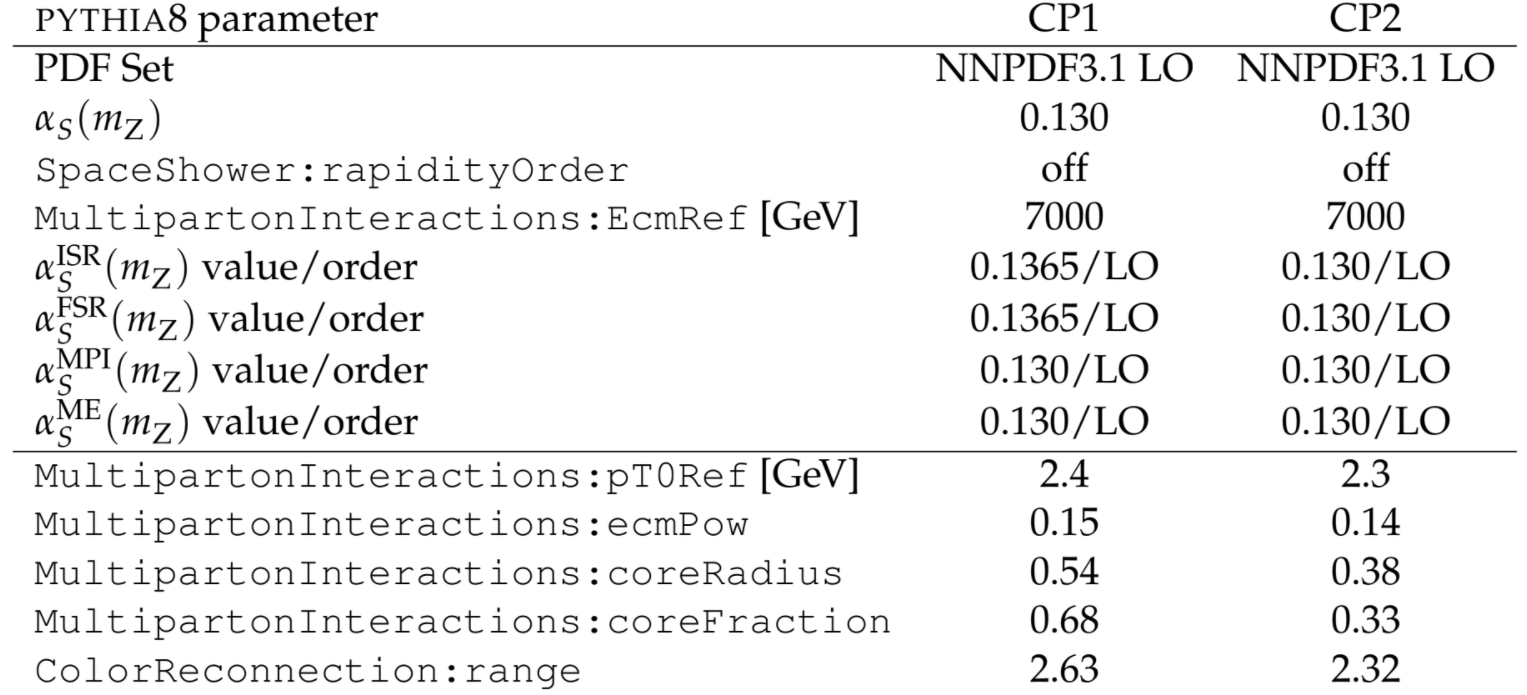
\includegraphics[width=0.95\textwidth]{{img/CPtunes1.png}}
	\caption{CP1 and CP2 tunes settings are report here together with the values for the parameters tuned. CP1 and CP2 use a LO PDF set. CP1 $\alpha_s$ is different between matrix element calculation and MPI that use a value of 0.1365 ISR and FSR that instead use 0.130. While, CP2 use the same value for all processes, it is fixed at 0.130. In both cases $\alpha_s$ run with a LO evolution. Table from \cite{CPtunes}}
	\label{fig:CPtunes1}
\end{table}

\begin{table}[!ht]
	\centering
	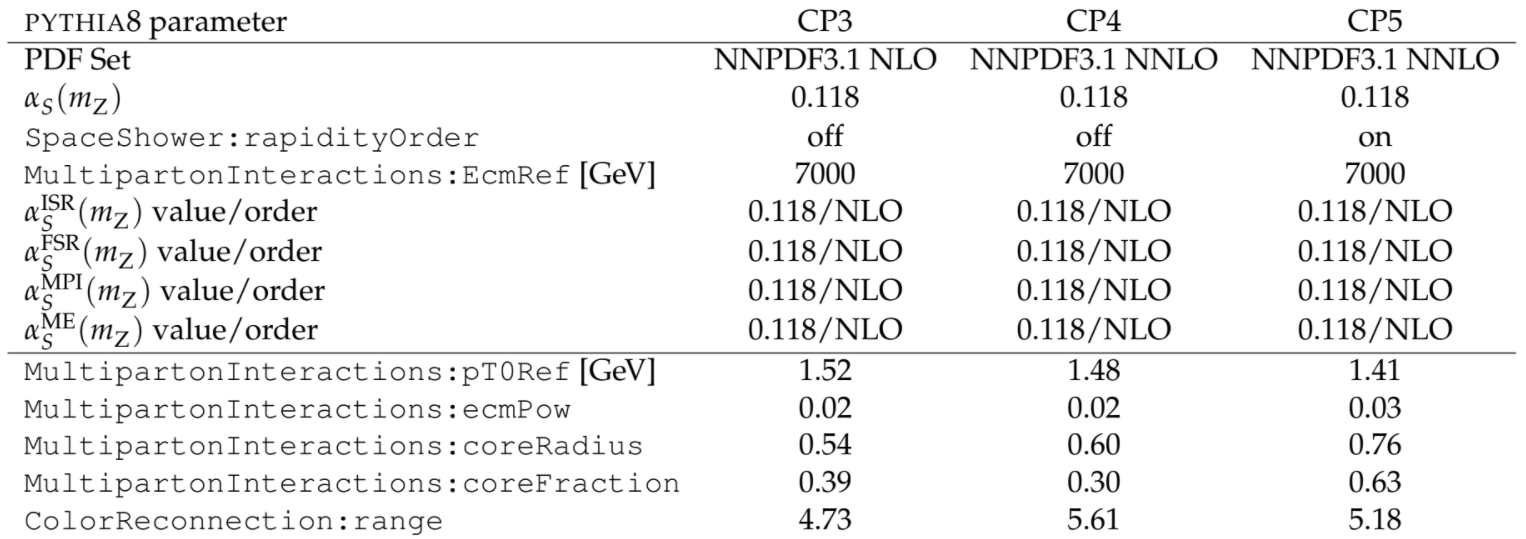
\includegraphics[width=0.95\textwidth]{{img/CPtunes2.png}}
	\caption{here are reported CP3, CP4 and CP5 tunes settings, and the results for the tune. The three tunes use an equal $\alpha_s$ value for al the processes, $\alpha_s=0.118$ running with a NLO evolution. The difference between CP3 and the other two tune is that CP3 use a NLO PDF set while CP4 and CP5 a NNLO one. CP5 ISR emission is also ordered according to rapidity. Table from \cite{CPtunes}}
	\label{fig:CPtunes2}
\end{table}

Below we are going to focus on CP5 tune. We are going to reproduce this tune using the same settings for \texttt{pythia8} but using a different tuning software: \texttt{mcnntunes}. In the next section \texttt{mcnntunes} working mode is explained. 

\section{MCNNTUNES}

\texttt{mcnntunes} \cite{MCNNTUNESarticle} is a Shower Monte Carlo generators tuning tool,  that implement a tune procedure based on the use of Feed Forward Neural Networks (FFNNs). The advantage of using FFNNs have been described above and is that they are universal function approximators. This remove the polynomial bias present in \texttt{professor} tool.
\\
\texttt{mcnntunes} offers two different operation modes: \textit{PerBin Model} and \textit{Inverse Model}. The first one is based on approach similar to the one in \texttt{professor} but where the response of the generator is parameterized using these FFNNs; the later is a new approach where the NN is trained to infers the parameters value from the experimental values of the bins in the distributions used.
\\
In next two sections we are going to describe the two methods in details.

The two approach have the same starting point that is a sampling of the parameter space (e.g. for the UE analysis we use the parameters space shown in \tableRef{table:CP5variations}), than the generator is run with every sample. All these MC runs are going to build our dataset that is called \textit{training set}.

\subsection{Per Bin Model}

PerBin Model is a parametrisation-based method. The main idea, as shown in \figRef{fig:PerBinModel_schematic} is to build a model (i.e. a neural network) for each bin in order to parameterize the generator output. Each NN takes the parameters values as input and return the bin value as output.
\\
All these NNs are then trained feeding the MC runs from the training set. All the training set are trained using a gradient-based algorithm, as usual for feed forward neural networks, with mean squared error as loss.
\\
Once, the NN is trained, the last step is the tune in which one actually get the best parameters.  This step define a surrogate loss function for the tuning problem. In fact, the parameterization step return a model $h^(i)(\mathbf{p})$ for each bin, $i$, and where $\mathbf{p}$ is the vector of the parameters. 
\\
Than this surrogate loss function defined as:
\begin{equation}
	\chi^2=\displaystyle\sum_{i=1}^N\frac{\left( h^{(i)}(\mathbf{p})-h_{exp}^{(i)}\right)^2}{\sigma_{(i)}^2}
\end{equation}
need to be minimized in order to evaluate the best estimation for the parameters. In \texttt{mcnntunes} this minimization is performed using the CMA-ES algorithm \cite{CMAES}.
\\
So the best estimation for the parameters is the configuration of parameters that minimize this $\chi^2$.  

\begin{figure}[!ht]
	\centering
	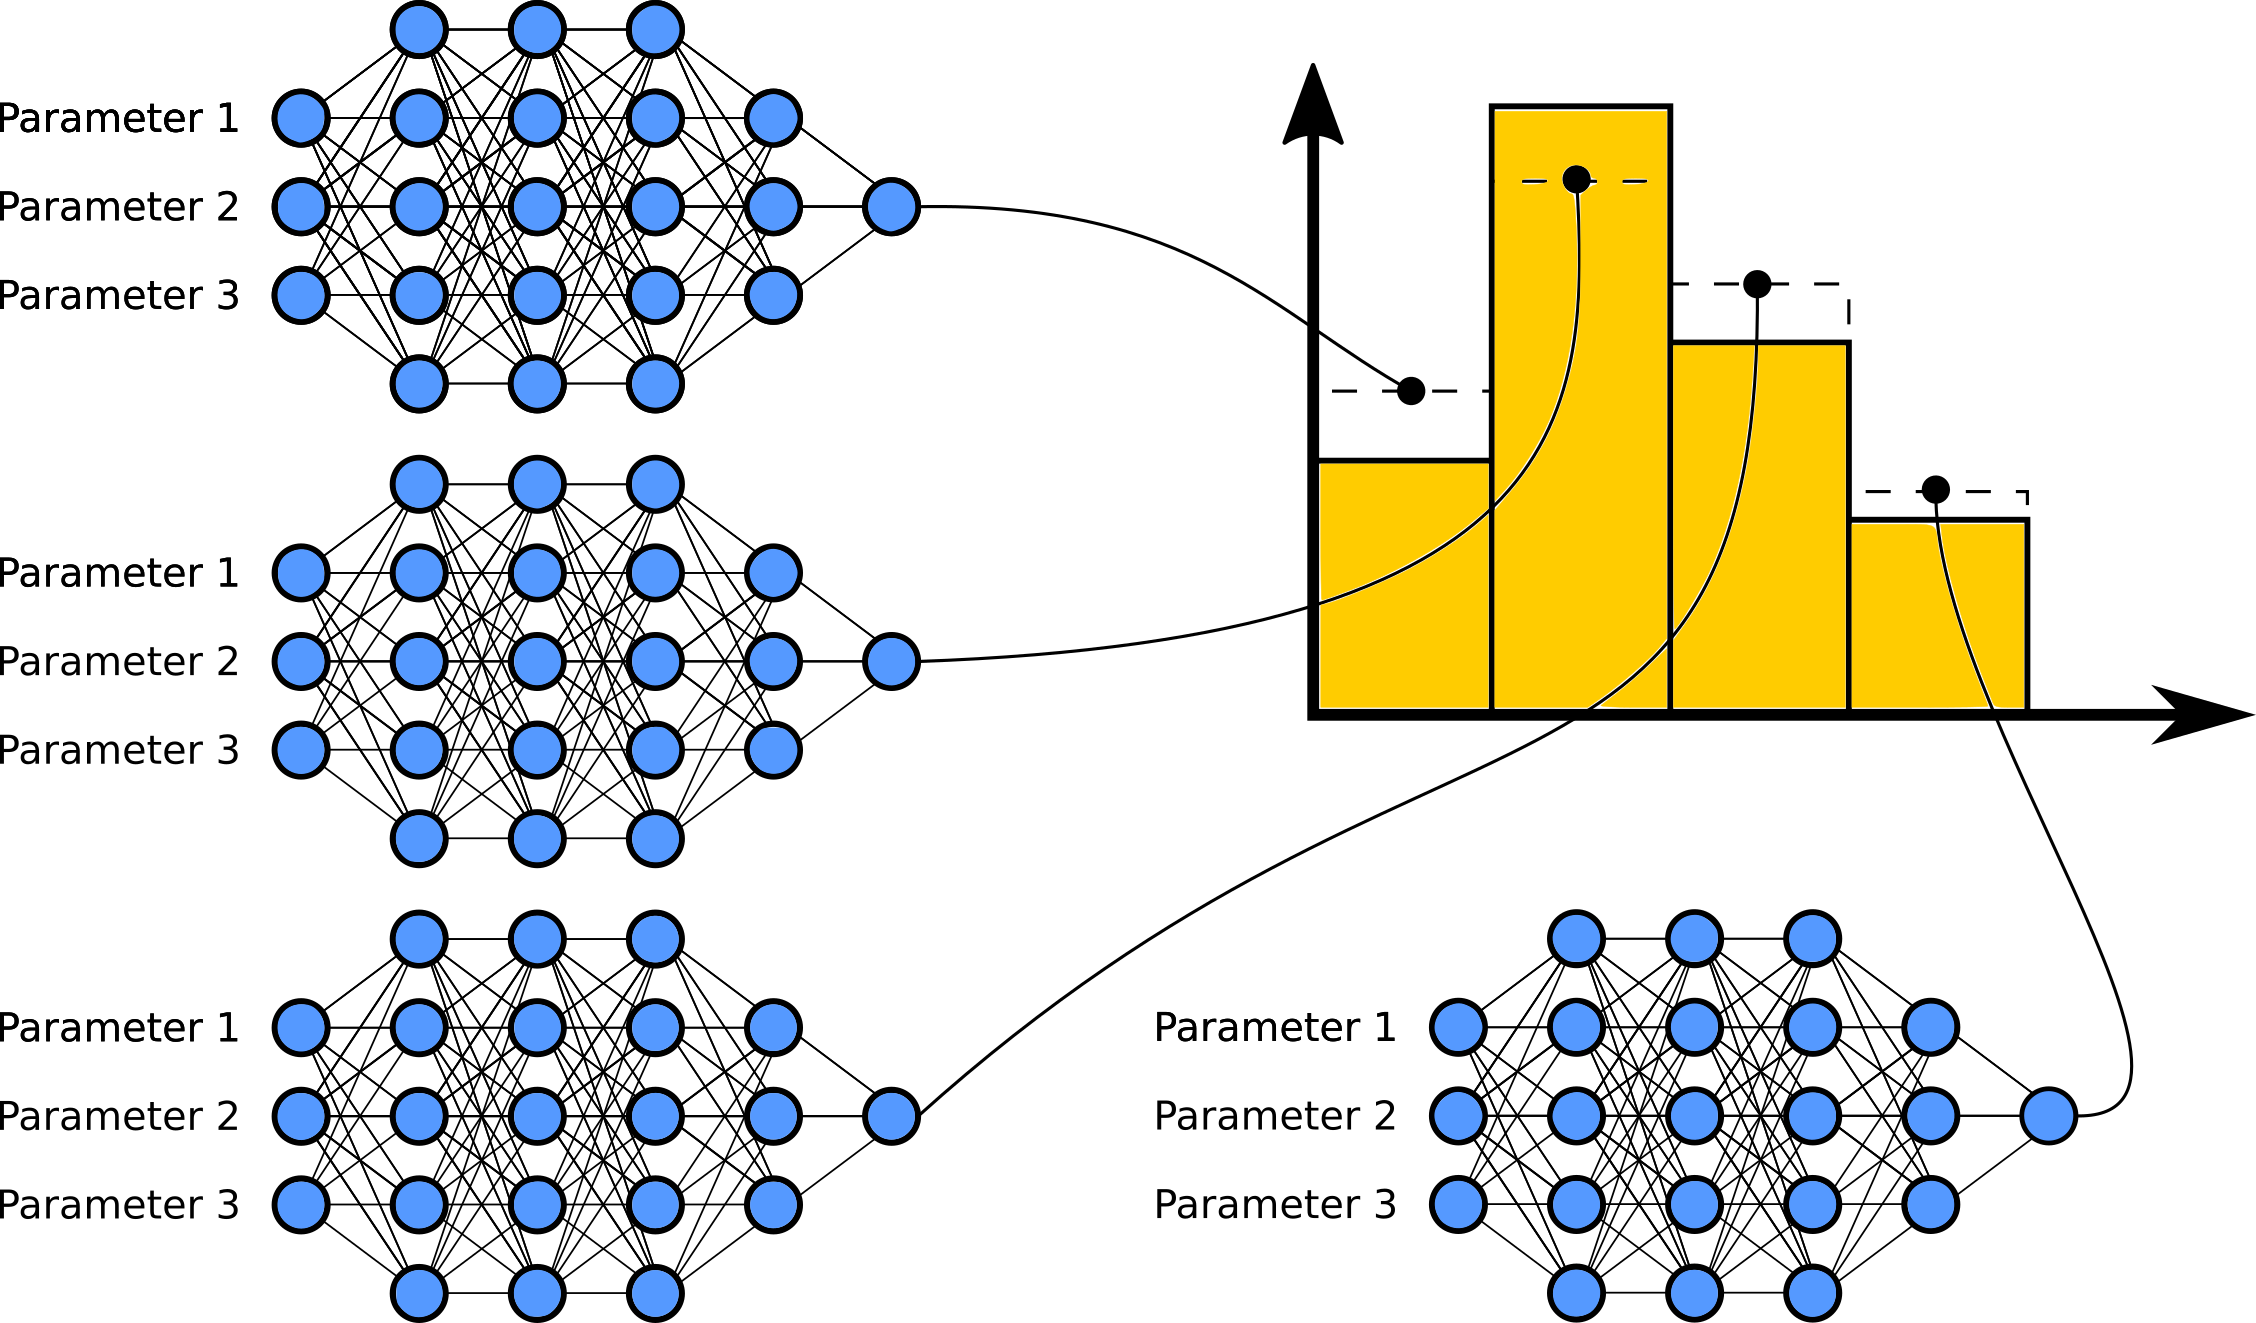
\includegraphics[width=0.8\textwidth]{{img/PerBinModel.png}}
	\caption{Figure from \cite{MCNNTUNESarticle}}
	\label{fig:PerBinModel_schematic}
\end{figure}

\subsubsection*{Errors evaluation}

The error evaluation for the PerBin Model is given by the definition of a confidence interval using the $\chi^2$ function.
In fact, as shown in section 9.6 and 9.7 of \cite{cowan}, for an estimators vector $\hat{h}(\mathbf{p})=(\hat{h}^{(1)}(\mathbf{p}),\hat{h}^{(2)}(\mathbf{p}),\dots,\hat{h}^{(n)}(\mathbf{p}))$ for the parameters $\hat{h}(\mathbf{p})$ the probability distribution function and the likelihood (the $\chi^2$ in our case) in limit of a large sample are Gaussian distributed. The probability distribution function for the estimators is 
\begin{equation}
f(\hat{h}(\mathbf{p})|h(\mathbf{p})) = \frac{1}{(2\pi)^{n/2}|V|^{1/2}}\exp\left[ -\frac{1}{2}\left(\hat{h}(\mathbf{p}) - h(\mathbf{p})\right)^T V^{-1} \left(\hat{h}(\mathbf{p}) - h(\mathbf{p})\right) \right] 
\end{equation}
where $T$ is the transpose vector and $V^{-1}$ is the inverse covariance matrix. 
Can be shown that also the likelihood is Gaussian as the probability distribution function. So a changing in the parameter give a calculable variation in the $\chi^2$
\begin{equation}
	\frac{\chi^2(\text{c.i.})}{N_{dof}}= \frac{\chi^2_{min}}{N_{dof}}+\frac{Q_\gamma}{N_{dof}}
	\label{eq:chi2_variation}
\end{equation} 
The variation is dependent on the number of parameters and on the chosen confidence level ($1\sigma=0.683$ in our case) and a list of the values is reported in \tableRef{table:percentile}.

\begin{table}
	\centering
	\begin{tabular}{c | c c c c c}
		\multirow{ 2}{*}{percentile} & \multicolumn{5}{c}{$Q_\gamma$}\\\cline{2-6}
		& $n=1$ & $n=2$ & $n=3$ & $n=4$ & $n=5$ \\\hline\hline
		$0.683$& $ 1.00 $ & $ 2.30 $ & $ 3.53 $ & $ 4.72 $ & $ 5.89 $ \\
		$0.90$ &  $ 2.71 $ & $ 4.61 $ & $ 6.25 $ & $ 7.82 $ & $ 9.24 $ \\
		$0.95$ & $ 3.84 $ & $ 5.99 $ & $ 7.82 $ & $ 9.49 $ & $ 11.1 $ \\
		$0.99$ & $ 6.63 $ & $ 9.21 $ & $ 11.3 $ & $ 13.3 $ & $ 15.1 $ \\
	\end{tabular}
	\caption{The table report the values of the quantile $Q_\gamma$ for different confidence level $0.683$ is the row corresponding to the $1\sigma$ definition and is the one of our interest.}
	\label{table:percentile}
\end{table}

Then, the error is defined as the value of the parameters that give a deviation from the minimum value of the $\chi^2/N_{dof}$ equal to the $Q_\gamma/N_{dof}$ value for a confidence level of $0.683$, as defined in \eqRef{eq:chi2_variation}. An example for the evaluation in \texttt{mcnntunes} is shown in \figRef{fig:exampleChi2Variation} where the green line is the quantities defined here in \eqRef{eq:chi2_variation} and the errors are given by the intersections between this line and the blue line, that is the $chi^2/N_{dof}$ for the different values of the parameter.

\begin{figure}[!ht]
	\centering
	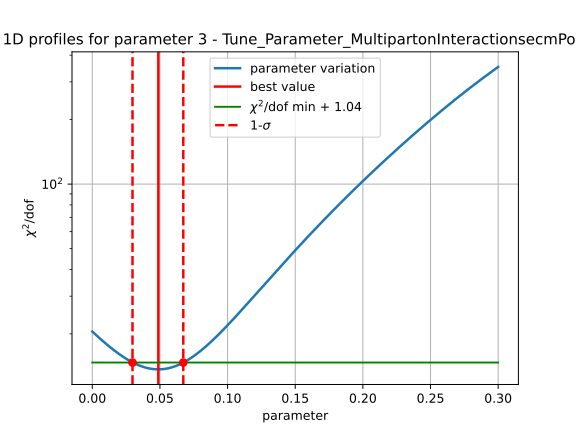
\includegraphics[width=0.6\textwidth]{{img/exampleChi2Variation.png}}
	\caption{This figure shows the error evaluation in \texttt{mcnntunes} for the \texttt{MultipartonInteractions:ecmPow} \texttt{Pythia8} parameter. The blue line is the value of the $\chi2/N_{dof}$ evaluated for different parameter values. The best estimation is indicated by the vertical red line, while the green line is the quantity in \eqRef{eq:chi2_variation}. The error is evaluated from the intersection of blue and green lines.
	}
	\label{fig:exampleChi2Variation}
\end{figure}

\subsection{Inverse Model}

The Inverse Model is the most innovative tuning procedure introduced by \texttt{mcnntunes}. This model contrarily to the PerBin Model takes the histograms bins as input and returns parameters values as output. For the Inverse Model the NN used is only one as shown schematically in \figRef{fig:InverseModel_schematic}. What the Inverse Model try to do is to learn the inverted model of the generator. So starting from the observed values the model try to reproduce the parameters values necessary to get the histograms we use as input.

The model is build and then trained with the training set introduced before. Once the model is trained feeding the experimental data to the NN this can try to infer the values of the parameters required to get the output. 

\begin{figure}[!ht]
	\centering
	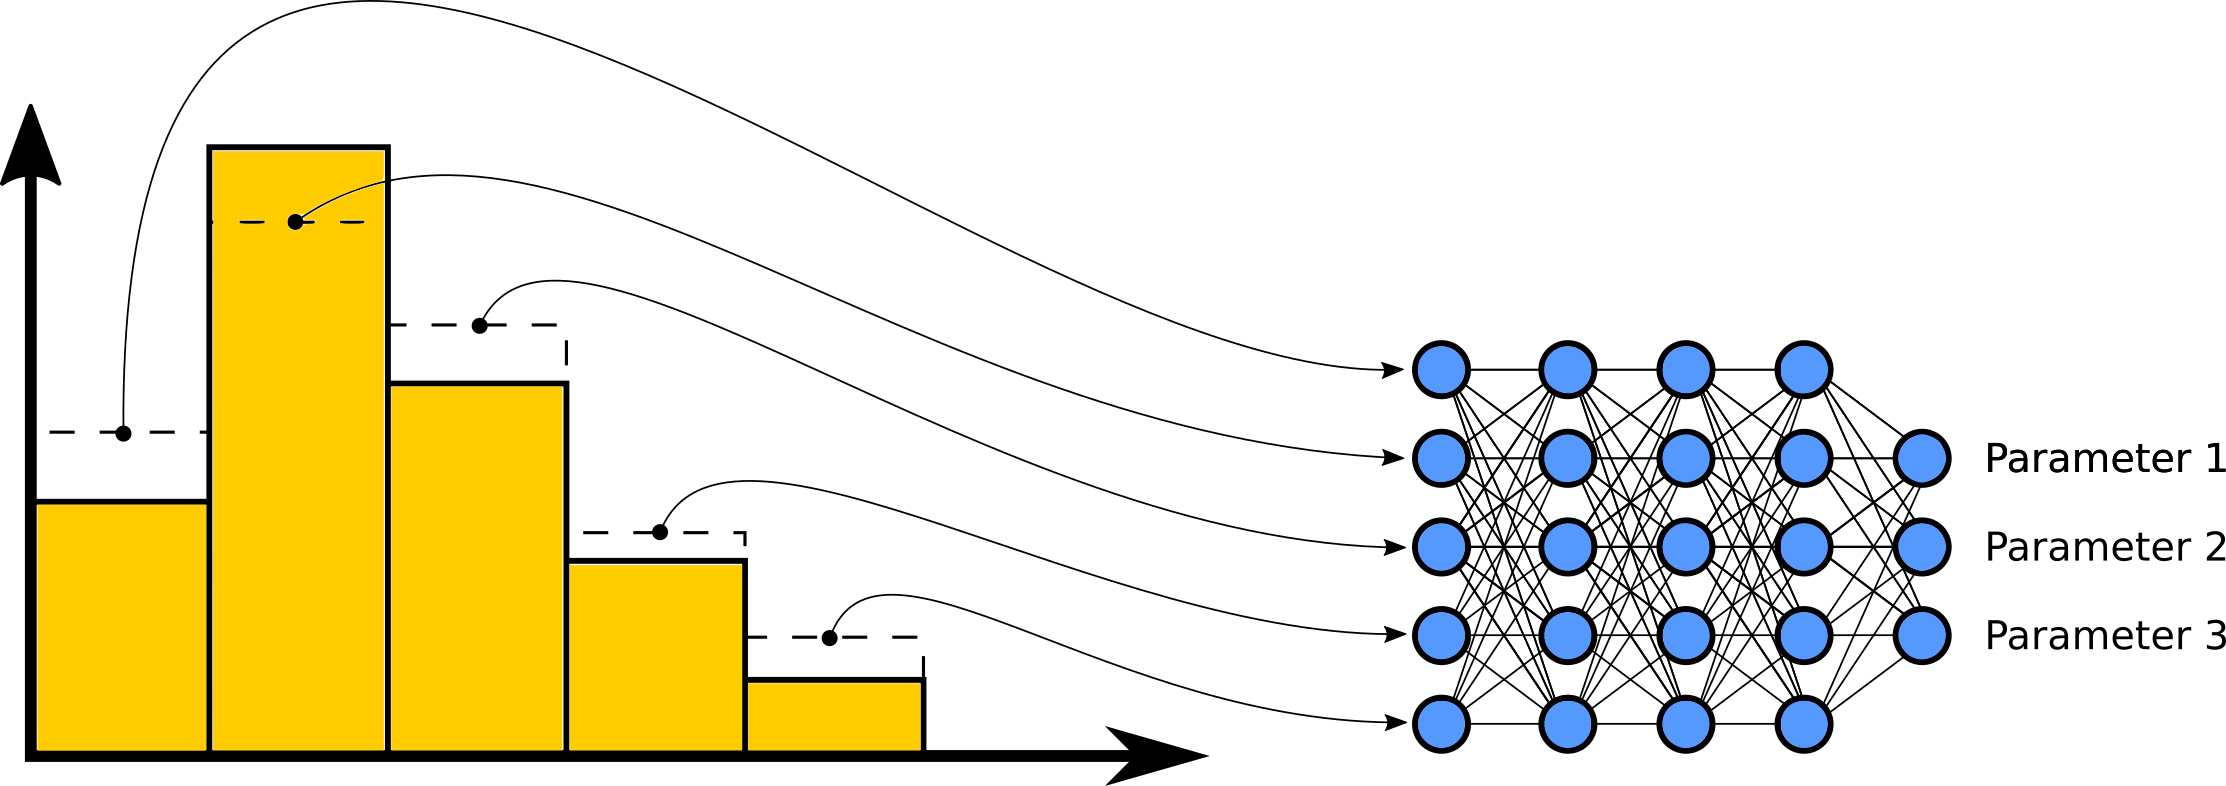
\includegraphics[width=0.8\textwidth]{{img/InverseModel.png}}
	\caption{Figure from \cite{MCNNTUNESarticle}}
	\label{fig:InverseModel_schematic}
\end{figure}

\subsubsection*{Errors evaluation}

The errors are evaluated in a different way respect to PerBin Model in fact in the Inverse Model there is not a minimization step, and the error is evaluated by a re-sampling of the experimental data using a \textit{multivariate Gaussian Distribution}, as in \eqRef{eq:gaussianDristribution} with a diagonal covariance matrix that have experimental uncertainties on the main diagonal.
\begin{equation}
	f(x_i; h^{(i)}_{\text{exp}}, \sigma^{(i)}_{\text{exp}})\,=\,\mathcal{N}\cdot\exp\left[ 
	-\frac{1}{2}
	\displaystyle\sum_{j=1}^{N_{bins}}
	\frac{\left( 
	x_i - h^{(i)}_{\text{exp}} 
	\right)^2}{{\sigma^{(i)}_{\text{exp}}}^2} 
	\right]
	\label{eq:gaussianDristribution}
\end{equation}
So, a set of histograms is generated, then this is fed to the NN and a distribution of predictions is generated. An example is shown in \figRef{fig:InverseModel_predictionsSpread}, from this distribution one can compute the error by evaluating the standard deviation.

\begin{figure}[!ht]
	\centering
	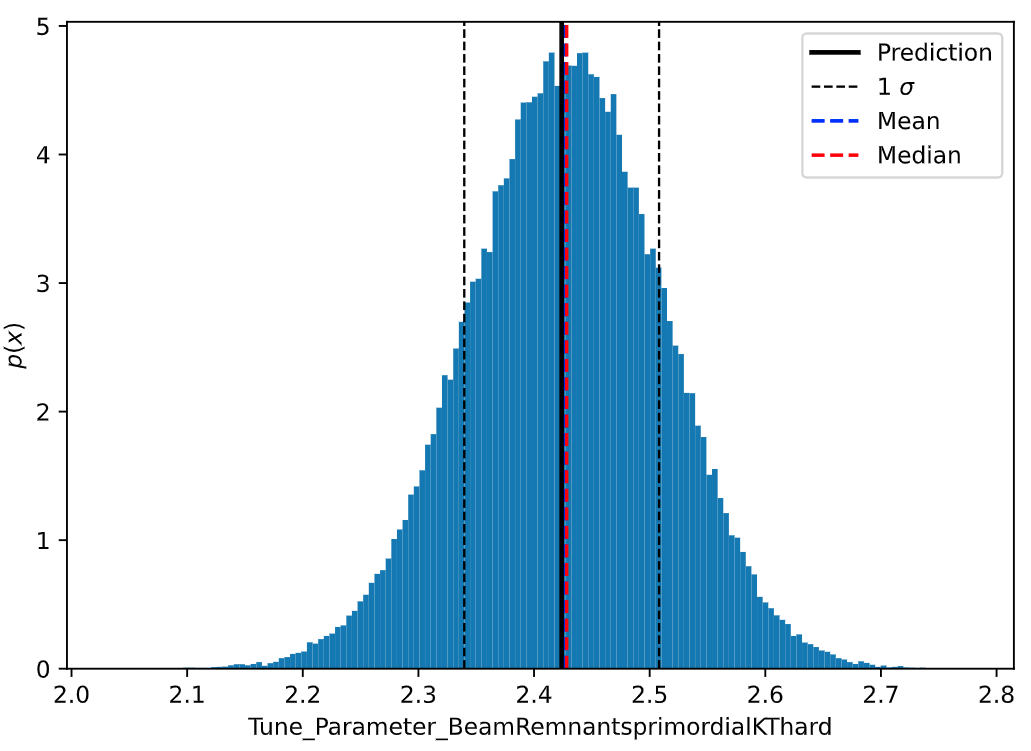
\includegraphics[width=0.6\textwidth]{{img/InverseModel_predictionsSpread.png}}
	\caption{Predictions spread for the inverse model after that a Gaussian resample is performed}
	\label{fig:InverseModel_predictionsSpread}
\end{figure}

Note that this is a new method for the tune
   

\subsubsection*{Hyperparameters}